\lecture{1.3}{Probability Foundations}
\label{lec:1-3}

\subsection{Joint Distributions}

Probability distributions describe how variables vary in a population. When more than one variable is considered at the same time, the relevant object is a joint distribution.

\begin{definition}[Joint distribution]
For discrete variables $X$ and $Y$, the \emph{joint distribution} assigns probabilities
\[
\Prob(X=x,Y=y)
\]
to every possible pair of values $(x,y)$. For continuous variables, the joint distribution is described by a joint density or by probabilities of regions.
\end{definition}

The joint distribution contains information about each variable separately and about how the variables relate to each other. If $A$ denotes monoclonal antibody receipt and $Y$ denotes HIV infection status, then
\[
\Prob(A=1,Y=1)
\]
is the proportion of the target population who both received monoclonal antibodies and are HIV infected.

If $W$ denotes age, then
\[
\Prob(W=65,A=1,Y=0)
\]
is the proportion of the population who are exactly 65 years old, received monoclonal antibodies, and are not HIV infected. For continuous age, one would usually use an interval such as $\Prob(65\le W<66,A=1,Y=0)$.

\subsection{Marginal Distributions}

A marginal distribution describes one variable or a subset of variables without conditioning on the remaining variables.

\begin{definition}[Marginal distribution]
For discrete variables $X$ and $Y$, the marginal distribution of $X$ is obtained from the joint distribution by summing over all possible values of $Y$:
\[
\Prob(X=x)=\sum_y \Prob(X=x,Y=y).
\]
\end{definition}

This operation is called marginalization. It removes a variable by adding over its possible values.

\begin{example}[Marginalizing over treatment]
Let $Y$ be HIV infection status and $A$ be monoclonal antibody receipt. The population prevalence of HIV infection is
\[
\Prob(Y=1)
=\Prob(Y=1,A=0)+\Prob(Y=1,A=1)
=\sum_{a=0}^1 \Prob(Y=1,A=a).
\]
The total infected group is partitioned into infected nonrecipients and infected recipients.
\end{example}

\begin{figure}[H]
\centering
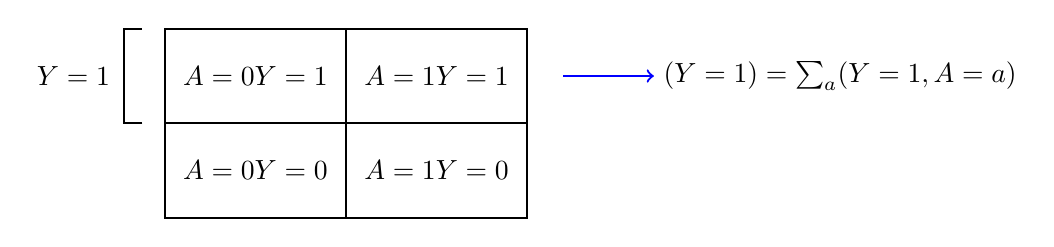
\begin{tikzpicture}[x=1.15cm,y=0.8cm]
  \draw[thick] (0,0) rectangle (4,3);
  \draw[thick] (2,0) -- (2,3);
  \draw[thick] (0,1.5) -- (4,1.5);
  \node at (1,2.25) {$A=0$\\$Y=1$};
  \node at (3,2.25) {$A=1$\\$Y=1$};
  \node at (1,.75) {$A=0$\\$Y=0$};
  \node at (3,.75) {$A=1$\\$Y=0$};
  \draw[thick] (-.25,1.5) -- (-.45,1.5) -- (-.45,3) -- (-.25,3);
  \node[left] at (-.5,2.25) {$Y=1$};
  \draw[->, thick, blue] (4.4,2.25) -- (5.4,2.25);
  \node[right] at (5.4,2.25) {$\Prob(Y=1)=\sum_a \Prob(Y=1,A=a)$};
\end{tikzpicture}
\caption{A marginal probability is obtained by adding joint probabilities over the variables being removed.}
\end{figure}

\subsection{Conditional Distributions}

Conditional probability describes a distribution inside a subgroup.

\begin{definition}[Conditional distribution]
For discrete variables $X$ and $Y$ with $\Prob(Y=y)>0$,
\[
\Prob(X=x\given Y=y)
=
\frac{\Prob(X=x,Y=y)}{\Prob(Y=y)}.
\]
\end{definition}

The denominator restricts attention to the subgroup with $Y=y$. The numerator counts the part of that subgroup that also has $X=x$. Thus conditional probability is a subgroup proportion.

\begin{example}[HIV infection among monoclonal recipients]
The probability of HIV infection among monoclonal antibody recipients is
\[
\Prob(Y=1\given A=1)
=
\frac{\Prob(Y=1,A=1)}{\Prob(A=1)}.
\]
This is not the fraction infected in the whole population. It is the fraction infected among the recipient subgroup.
\end{example}

With covariates, conditioning can define very specific subgroups. If $W=(W_1,W_2,W_3)$ represents age, BMI, and profession, then $W=w=(65,28.5,\text{nurse})$ defines the subgroup of 65-year-old nurses with BMI 28.5. A probability such as
\[
\Prob(Y=1\given A=1,W=w)
\]
is the probability of infection among monoclonal recipients in that covariate-defined subgroup.

\subsection{Chain Rule Factorization}

The definition of conditional probability can be rearranged to express a joint distribution as a product.

\begin{proposition}[Chain rule for two variables]
If $\Prob(X=x)>0$ and $\Prob(Y=y)>0$, then
\[
\Prob(X=x,Y=y)
=\Prob(X=x)\Prob(Y=y\given X=x)
=\Prob(Y=y)\Prob(X=x\given Y=y).
\]
\end{proposition}

\begin{proof}
By the definition of conditional probability,
\[
\Prob(Y=y\given X=x)
=\frac{\Prob(X=x,Y=y)}{\Prob(X=x)}.
\]
Multiplying both sides by $\Prob(X=x)$ gives
\[
\Prob(X=x)\Prob(Y=y\given X=x)=\Prob(X=x,Y=y).
\]
The second factorization follows by the same argument with $X$ and $Y$ interchanged.
\end{proof}

For three variables, repeated application gives
\[
\Prob(W=w,A=a,Y=y)
=
\Prob(W=w)\Prob(A=a\given W=w)\Prob(Y=y\given A=a,W=w).
\]
This factorization is a purely probabilistic identity. It does not by itself imply any causal ordering.

\subsection{Bayes Rule}

Bayes rule follows by combining the two chain rule factorizations.

\begin{proposition}[Bayes rule]
If $\Prob(Y=y)>0$, then
\[
\Prob(X=x\given Y=y)
=
\frac{\Prob(Y=y\given X=x)\Prob(X=x)}{\Prob(Y=y)}.
\]
Moreover,
\[
\Prob(Y=y)=\sum_x \Prob(Y=y\given X=x)\Prob(X=x)
\]
in the discrete case.
\end{proposition}

\begin{proof}
The chain rule gives
\[
\Prob(X=x,Y=y)=\Prob(Y=y\given X=x)\Prob(X=x).
\]
Substitute this expression into the definition
\[
\Prob(X=x\given Y=y)=\frac{\Prob(X=x,Y=y)}{\Prob(Y=y)}
\]
to obtain Bayes rule. The expression for $\Prob(Y=y)$ follows by marginalizing over $X$ and then applying the chain rule:
\[
\Prob(Y=y)
=\sum_x\Prob(X=x,Y=y)
=\sum_x\Prob(Y=y\given X=x)\Prob(X=x).
\]
\end{proof}

\subsection{From Joint to Marginal Probabilities}

The operation from joint to marginal probabilities is adding or integrating. For discrete variables,
\[
\Prob(X=x)=\sum_y \Prob(X=x,Y=y).
\]
For continuous variables with joint density $f_{X,Y}$,
\[
f_X(x)=\int f_{X,Y}(x,y)\,dy.
\]
The same principle applies to mixed or higher-dimensional data. For example,
\[
\Prob(W=25,A=1)
=
\sum_{y=0}^1 \Prob(W=25,A=1,Y=y),
\]
and
\[
\Prob(W=25)
=
\sum_{a=0}^1\sum_{y=0}^1 \Prob(W=25,A=a,Y=y).
\]

The idea is simple: to ignore a variable, add over every way that variable could have occurred.

\subsection{Conditional Probability as Subgroup Proportion}

The most important intuition in this lecture is that conditioning defines a subgroup.

\begin{keyidea}
Conditional probability equals a proportion within a subgroup:
\[
\Prob(\text{characteristic}\given \text{subgroup})
=
\frac{\Prob(\text{characteristic and subgroup})}
{\Prob(\text{subgroup})}.
\]
\end{keyidea}

For instance,
\[
\Prob(Y=1\given W=25,A=1)
=
\frac{\Prob(Y=1,W=25,A=1)}{\Prob(W=25,A=1)}.
\]
The denominator is the proportion of the whole population who are 25-year-old monoclonal recipients. The numerator is the proportion of the whole population who are 25-year-old monoclonal recipients and HIV infected. Dividing converts the whole-population proportion into a within-subgroup proportion.

This subgroup interpretation will be used constantly in causal inference. When we later write expressions such as $\E(Y\given A=1,W=w)$ or $\Prob(A=1\given W=w)$, the conditioning variables define the subgroup in which an outcome mean or treatment probability is being described.
